%!TEX root = ../Thesis.tex
%!TEX program = xelatex
\documentclass[../Thesis]{subfiles}


% 本文
\begin{document}
\chapter{手法}
\section{概要}
  提案手法の概要図を\fref{img01}に示す.提案手法では、入力画像であるドローン空撮映像を分割したフレーム画像に対し前処理として領域分割とヒストグラム均一化を行い、色情報や土地被覆指標等を用いて斜面崩壊、浸水領域を検出する。次に、これらの領域から植生、空、瓦礫、建物領域を除去し最終出力結果とする。
  	
	\begin{figure}[h]
		\centering
		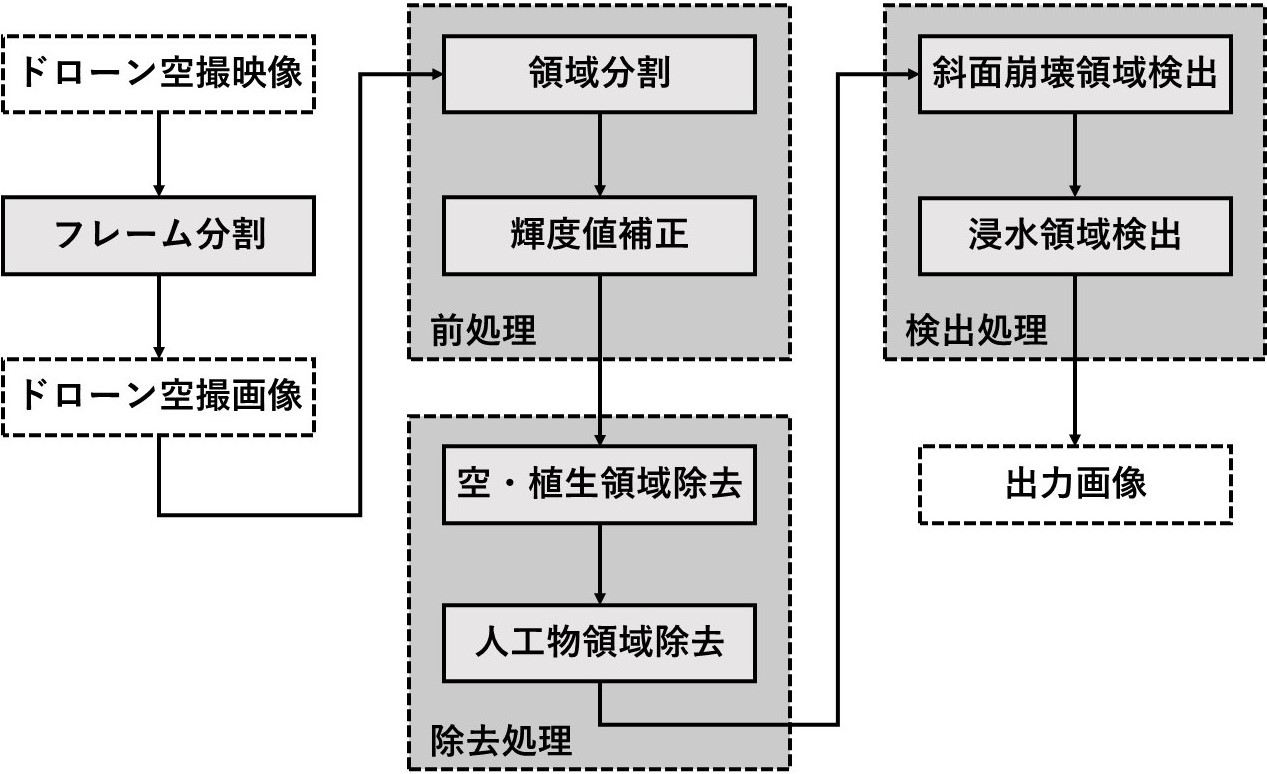
\includegraphics[width=8cm]{img/howto3.jpg}
		\caption{提案手法概要図}
		\label{img01}
  \end{figure}
  

\section{領域分割}
  斜面崩壊・浸水領域を画素単位で検出することは難しいため、近傍画素との関係性を考慮した上で領域単位で判別を行う。本研究ではMean-Shift法を用いた領域分割を行う。Mean-Shift法はカーネル密度推定によるクラスタリング手法の一つで画像の領域分割、動画像における対象物体追跡に用いられる。また、領域分割の代表的な手法であるk-means法に比べ、クラスタ数を事前に決める必要が無い。d次元空間中のN個の点群$x_i$を標本として得られるような確率密度関数$f(x)$を考え、その標本点から確率密度関数$f(x)$の極大点を探索する手法である。
  次に、Mean-Shift法にてカラー画像の領域分割を行う手順について説明する。

  \begin{enumerate}
    \item カラー画像中の各画素の位置を二次元座標$x_i$、その画素値を三次元チャンネル$v_i=(R_i,G_i,B_i)$とし、画素位置と画素値を結合した5次元空間内の点$z_i=(x_i,v_i)$を考える。距離と色相が近い画素が5次元空間内でクラスタを成しているとし、各画素をMean-Shift法でクラスタリングする。
    \item 画素位置、画素値のバンド幅をそれぞれ$h_s,h_r$とする。すべての$z_i$にMean-Shift法を適用し、収束位置$z^c=(x^c,v^c)$を計算する。
    \item $x_i$の画素値を収束位置の画素の値$v_i=(R_i,G_i,B_i)$に置き換えることによって領域分割ができる。
  \end{enumerate}
  
  なお、$x^s,x^r$をそれぞれ5次元ベクトルの空間に対応するものとし、カーネル密度推定を以下{式x}のように定義することでMean-Shift法は以下のように計算される。

  \begin{equation}
    f(x) = \frac{c}{Nh_s^2h_r^3} \sum_{i=1}^N k (|\frac{x^s-x_i^s}{h_s}|^2) k (|\frac{x^r-x_i^r}{h_r}|^2)
  \end{equation}

  \begin{equation}
    y_{j+1}^s = \frac{\sum_{i=1}^N g_i^sx_i^s}{\sum_{i=1}^N g_i^s}, y_{j+1}^r = \frac{\sum_{i=1}^N g_i^rx_i^r}{\sum_{i=1}^N g_i^s}
  \end{equation}

  ただし、
  \begin{equation}
    g_i^s = k' (|\frac{y_j^s-x_i^s}{h_s}|^2) k (|\frac{y_i^r-x_i^r}{h_r}|^2), g_i^r = k (|\frac{y_j^s-x_i^s}{h_s}|^2) k' (|\frac{y_i^r-x_i^r}{h_r}|^2)
  \end{equation}
  である。
  
  なお、本研究ではMean-Shift法の特徴量空間に距離を表す画素位置(x,y)、色相を表す画素値(R,G,B)を用いるので5次元空間での処理となり、距離、色相の近しい画素郡が一つの領域となる。領域分割の実行結果を\fref{img02}に示す。

  \begin{figure}[h]
		\centering
		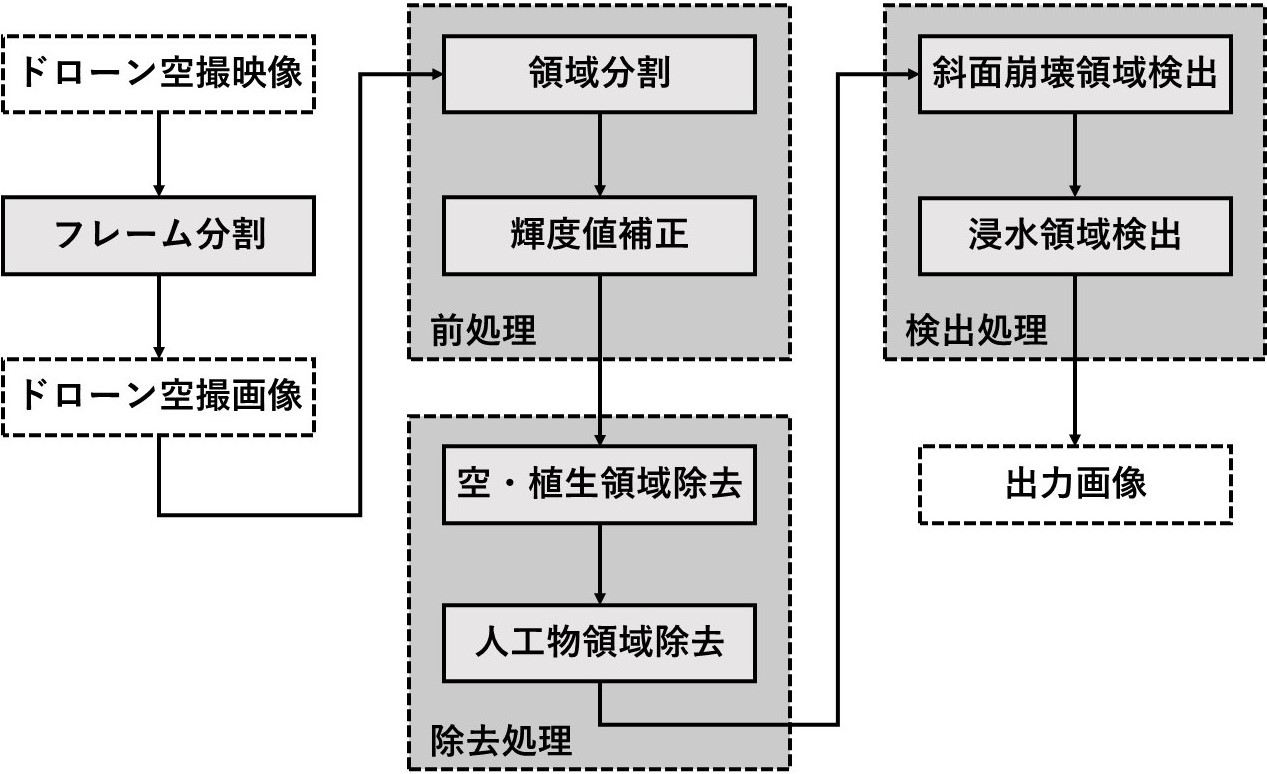
\includegraphics[width=8cm]{img/howto3.jpg}
		\caption{領域分割}
		\label{img02}
  \end{figure}


\section{ヒストグラム均一化}
  空撮画像は撮影時の天候や時刻、季節によって色相や輝度に偏りが生じる。本研究では色相や輝度、色情報を用いた指標によって判別処理を行うので偏りによって検出結果に影響が生じる可能性があるのでCLAHEのアルゴリズムによってヒストグラムを均一化する。\cite{art05}。CLAHEのアルゴリズムとは画像をタイルと呼ばれる小領域に分割し、タイル毎にヒストグラム均一化を行う手法である。ただし、タイル毎に均一化を行うとノイズが強調されるため、ビンの出現頻度が特定の上限値以上となった場合、その画素をその他のビンに均等に配分した後ヒストグラムの均一化を行うことによってノイズの強調を抑える。よって、本研究ではCLAHEのアルゴリズムによってノイズの強調を抑えつつヒストグラムの均一化を行う。ヒストグラム均一化の実行結果を\fref{img03}に示す。

	\begin{figure}[h]
		\centering
		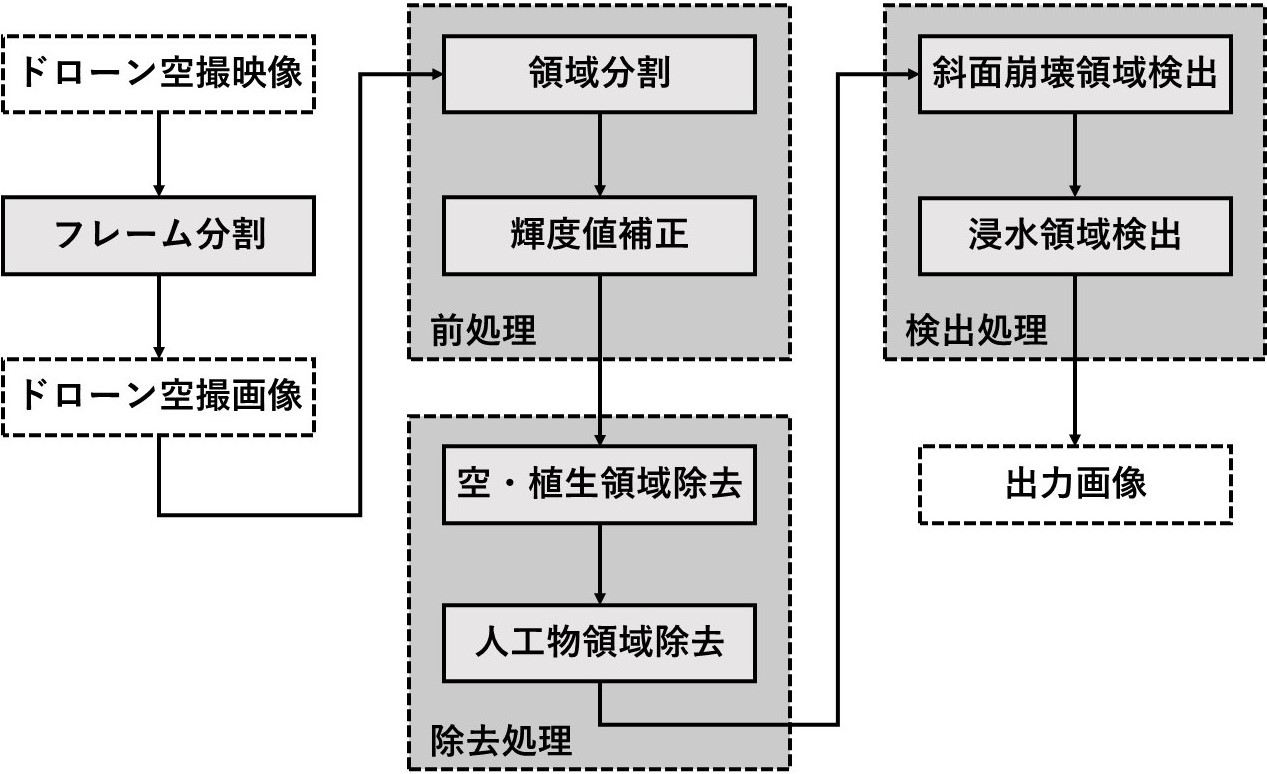
\includegraphics[width=8cm]{img/howto3.jpg}
		\caption{ヒストグラム均一化}
		\label{img03}
  \end{figure}


\section{災害領域検出}
% \section{斜面崩壊・浸水領域検出}
  斜面崩壊・浸水領域での色情報や輝度情報等の特徴を\tref{tab01}に示す。

  斜面崩壊と浸水が重複した場合どうしようっっs
    
  \begin{table}[h]
    \centering
    \caption{各災害領域の特徴}
    \label{tab01}
    \begin{tabular}{l l l l l l}
      領域名 & L* & a* & b* & S & dis \\
      \hline
      \hline
      斜面崩壊 & 低い & 高い & - & 高い & 高い \\
      浸水 & 高い & 高い & - & 低い & 低い \\
    \end{tabular}
  \end{table}

\subsection{L*a*b*表色系変換}
  前述の各災害領域の特徴に従って分類を行うためヒストグラム均一化を行った画像に対しL*a*b*表色変換を行う。L*a*b*表色系とは輝度をL*、色相と彩度を示す色度をa*,b*で表した色空間である。また、人間の視覚に近い色空間であり、色情報にて分類を行う際に有効な指標である。本研究で用いている画像は現時点ではRGB表色系にて表されているためL*a*b*表色系への変換を行う。RGB表色系からL*a*b*表色系への変換式を{}~{}に示す。なお、RGB表色系はデバイス依存色でありから直接L*a*b*表色系に変換する式は存在しないためデバイス独立色であるXYZ表色系に変換してから処理を行う。XYZ表色系への変換は0から255までの8bit値を0から1に変換し、γ=2.2に対するガンマ補正を線形の測定値に戻す。
  
  なお、EはR,G,Bのいずれかを表し、ダッシュ付きはガンマ補正された値を示す。
  
  \begin{equation}
    L* = 116 \times f(\frac{Y}{Y_n}) - 16
    a* = 500 \times f(\frac{X}{X_n}) - f(\frac{Y}{Y_n}))
    b* = 200 \times f(\frac{Y}{Y_n}) - f(\frac{Z}{Z_n}))
  \end{equation}
  \begin{equation}
    X = 0.4124R+0.3576G+0.1805R
    Y = 0.2126R+0.7152G+0.0722R
    Z = 0.0193R+0.1192G+0.9505R
  \end{equation}

  ただし、
  \begin{equation}
    E' = E'_{8bit}/255.0
    E = E'/12.92 E'<=0.04045
    ((E'+0.055)/1.055^2.4) E'>0.04045
  \end{equation}
  
  \begin{equation}
    f(t) = 
    t^{\frac{1}{3}} t>(\frac{6}{29}^3) \\
    \frac{1}{3}(\frac{29}{6})^2t+\frac{4}{29} t<=(\frac{6}{29}^3)
  \end{equation}
  とする。

\subsection{HSV表色系変換}
  前項同様ヒストグラム均一化を行った画像に対しHSV表色系変換を行う。HSV表色系とは色相(Hue),彩度(Saturation),明度(Value)の三成分からなる色空間でありこれらの成分を用いて分類を行う際に有効な指標である。よって、RGB表色系で表されたヒストグラム均一化画像に対しHSV表色系変換を行う。RGB表色系からHSV表色系への変換式を{}~{}に示す。なお、R,G,Bは0から1の範囲に正規化してあるとする。

  \begin{equation}
    E = E / 255.0
    Max = Max(R,G,B)
    Min = Min(R,G,B)
    H = \frac{G-B}{Max-Min} \times 60 Max = R
    H = \frac{B-R}{Max-Min} \times 60 + 120 Max = G
    H = \frac{R-G}{Max-Min} \times 60 + 240 Max = B
    H = 0 Max = Min
    S = Max - Min
    V = Max
  \end{equation}

\subsection{テクスチャ解析}
  前項同様xxxxx画像に対しテクスチャ解析を行う。テクスチャ解析とは画像内の領域を輝度パターンによって特徴付ける処理であり、リモートセンシングで土地被覆の分類に用いられることがある。本研究ではテクスチャの統計的特徴量を求めるために離れた2つの場所にある画素対の値から画素値の一様性、方向性、コントラストなどの表す特徴量を求める同時正規行列を用いる。
  次に、同時正規行列の求め方について説明する。\fref{img00}に示すようなある画素iとjの画素対について相対的な距離をδ=<d,θ>とする。それぞれの画素値をL_i,L_jとし、画素値の対(L_i,L_j)が生じる出現頻度である同時正規行列H_δ(L_i,L_j)を考える。ここで、出現頻度の総数でH_δ(L_i,L_j)を正規化し確率に変換した同時正規行列をP_δ(L_i,_j)とする。デジタル画像ではd=1の場合θのとりうる値は0°,45°,90°,135°,180°,225°,270°,315°となる。図xに求め方例を示す。
  本研究では画層の不均一度を表す指標である異質度を用いる。異質度は周辺画素との差が大きいと値が大きくなる指標であり、土砂や瓦礫等の検出に有効な指標である。異質度を求める式を{}に示す。

	\begin{figure}[h]
		\centering
		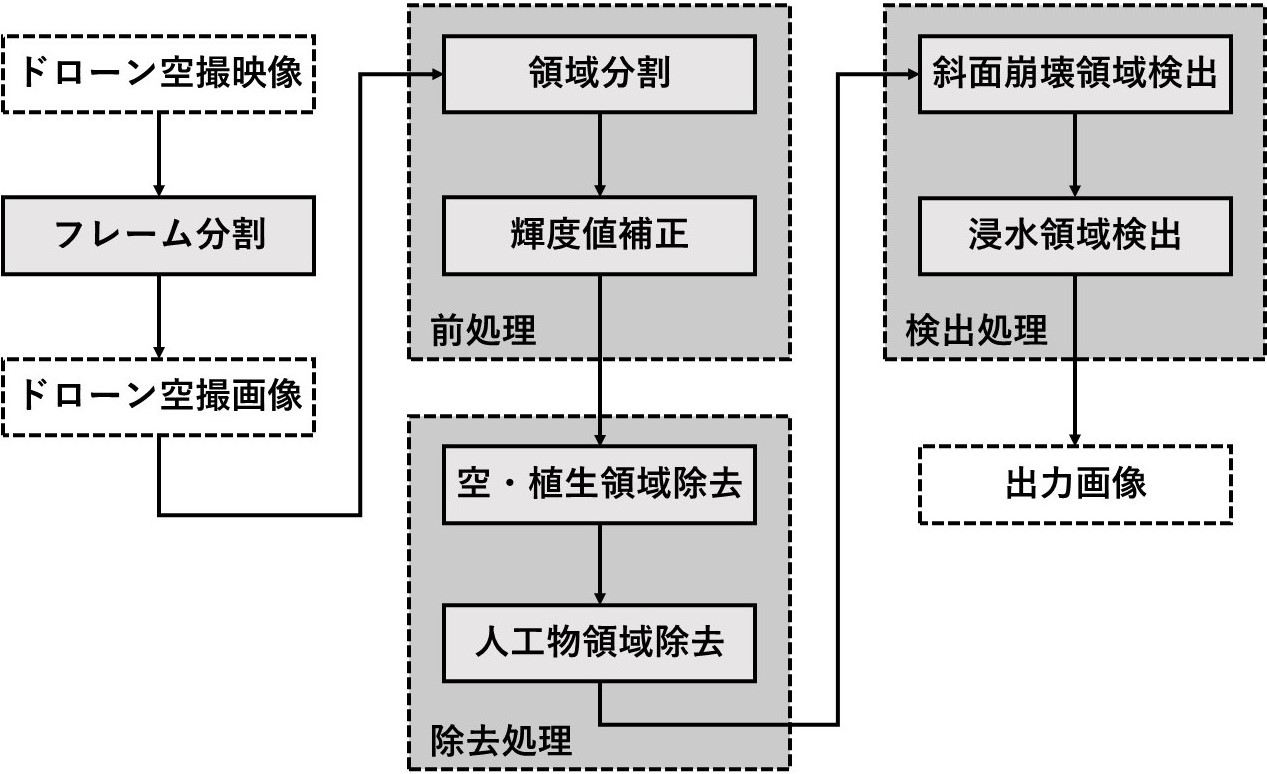
\includegraphics[width=8cm]{img/howto3.jpg}
		\caption{同時正規行列}
		\label{img00}
  \end{figure}

  \begin{equation}
    dissimilitarity = \frac{1}{2}(\sum_{255}^{i=0}\sum_{255}{j=0}P_{δ1}(i,j)|i-j|+\sum_{255}^{i=0}\sum_{255}{j=0}P_{δ2}(i,j)|i-j|)
    dissimilitarity = \sum_{255}^{i=0}\sum_{255}{j=0}P_δ(i,j)|i-j|
  \end{equation}

\subsection{斜面崩壊領域検出}


	斜面崩壊領域は赤色が強く,輝度が低いという特徴がある.また,土砂のような不均一な物質を多量に含むため,異質度が高い.これらの特徴を利用し色相,輝度,異質度により閾値処理を行う.

\subsection{浸水領域検出}
	浸水領域は赤色が強く,輝度が高いという特徴があるため2.6節と同様に閾値処理を行う.そして,これまでの処理を統合したものを最終出力結果とする.


\section{不要領域除去}
  最終出力結果にて誤検出を防ぐため空、植生、瓦礫、建物領域の除去を行う。各領域はそれぞれ\tref{tab01}のような特徴を持つため、この表に基づき色情報、輝度情報等にて各領域を検出する。検出したそれぞれの領域のマスク画像を作成し、災害領域検出結果よりマスクされた領域を除去し最終出力結果とする。

\begin{table}[h]
  \centering
  \caption{各災害領域の特徴}
  \label{tab01}
  \begin{tabular}{l l l l l l}
    領域名 & L* & a* & b* & IRR & dis \\
    \hline
    \hline
    空 & 高い & - & 低い & - & - \\
    植生 & 低い & 低い & 低い & - & - \\
    瓦礫 & - & - & - & - & 高い \\
    建物 & - & - & - & 高い & 低い \\
  \end{tabular}
\end{table}

\subsection{GSI}
% \subsection{エッジ抽出}
% \subsection{円形度}

\subsection{空領域検出}
  ドローンは撮影視点が横方向となることが多く画像中に空領域を含むことがある.空領域は青色が強く,輝度値が高いという特徴がある.L*a*b*表色系においてb*値が低いほど青色が強く,L*値が高いほど明るくなる.よって,L*a*b*表色系におけるb*値とL*値にて閾値処理を行い空領域を検出する。

\subsection{植生領域検出}
  山間部では頻繁に画像中に植生領域を含むため,誤検出低減のため空・植生領域を除去する.また,植生領域は緑色・青色が強いという特徴があるので,空領域と同様に閾値処理を行う.これらの閾値処理結果によりマスク画像を作成し,最終結果から除去する.
  
\subseciton{瓦礫領域検出}
  前節同様、誤検出を防ぐため瓦礫・建物領域の除去を行う。瓦礫・建物領域はそれぞれ表うんちのような特徴を持つため、この表に基づき瓦礫・建物領域を検出する。検出したそれぞれの領域のマスク画像を作成し、最終結果よりマスク領域を除去する。

  斜面崩壊,浸水,人工物領域は色相が類似していることが多く,2.4節のような色特徴での除去が難しい.そこで,本研究ではテクスチャ特徴量の指標の一つである異質度にて閾値処理を行う.異質度とは画像内の不均一度を示す指標であり,表面が不均一である程高い値を示す.2.4節同様,本処理結果を最終結果から除去する.
  
\subseciton{建物領域検出}

  均質な領域
  均質な領域尾を除去するかmの大大大

  斜面崩壊,浸水,人工物領域は色相が類似していることが多く,2.4節のような色特徴での除去が難しい.そこで,本研究ではテクスチャ特徴量の指標の一つである異質度にて閾値処理を行う.異質度とは画像内の不均一度を示す指標であり,表面が不均一である程高い値を示す.2.4節同様,本処理結果を最終結果から除去する.

\end{document}
